\chapter{Behavioral Modeling} \label{ch:behavioralModeling}
\chapterquote{People must give and then receive. First give and then you will have all. But instead, people want to first have all and then think of giving. This is not the right way.}{Meher Baba}

\graphicspath{{Chapters/BehavioralModeling/Figures/}}
\lstinputpath{Codes-VHDL/Chapter-BehavioralModeling/VHDLCodes} %path is defined in mypreamble


%\section{Introduction}
In this chapter, UART communication is discussed for NIOS design. Values of Sin(x) is generated using NIOS and the data is  received by computer using UART cable. Since, onchip memory is smaller for storing these values, therefore external memory i.e. SDRAM is used. Further, the received data is stored in a file using `Tera Term' software; finally live-plotting of data is performed using Python.  

In this chapter, we will learn following topics, 
\begin{enumerate}
	\item UART interface,
	\item Receiving the data on computer using UART communication,
	\item SDRAM interface,
	\item Saving data generated by NIOS desgin to a file using `Tera Term',
	\item Updating a existing QSys design and corresponding VHDL and NIOS design,
	\item Live-plotting of data using Python. 
\end{enumerate}

\section{UART interface}
First, create a empty project with name `UartComm' (see Section \ref{sec:new_project}). Next, open the QSys from Tools$\rightarrow$Qsys. Add `Nios Processor', `On-chip RAM (with 20k total-memory-size), `JTAG UART' and `UART (RS-232 Serial Port)' (\textbf{all with default settings}). Note that, Baud rate for UART is set to `115200' (see Fig. \ref{fig:uart_settings}), which will be used while getting the data on computer. Lastly, connect these items as shown in Fig. \ref{fig:uart_qsys_conn}; save it as `Uart\_Qsys.qsys' and finally generate the Qsys system and close the Qsys. Please see Section \ref{sec:CreateGenerateQsys}, if you have problem in generating the QSys system.

\begin{figure}[!h]
	\centering
	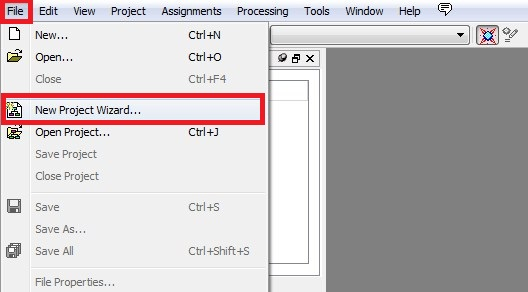
\includegraphics[scale=0.7]{1}
	\caption{UART settings}
	\label{fig:uart_settings}
\end{figure}
 
\begin{figure}[!h]
	\centering
	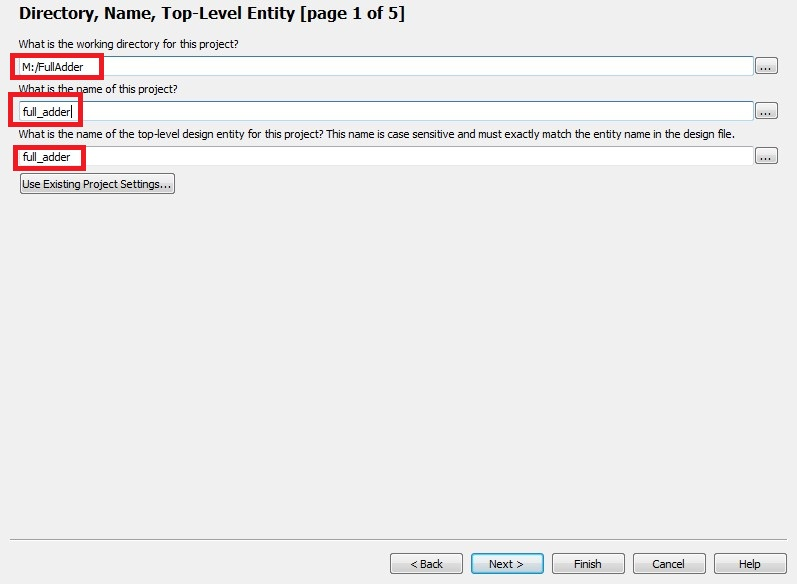
\includegraphics[scale=0.65]{2}
	\caption{Qsys connections}
	\label{fig:uart_qsys_conn}
\end{figure}

Now, add the file `Uart\_Qsys.qip' to the VHDL project. Next, create a new `Block diagram (.bdf) file and import the Qsys design to it and assign correct pin numbers to it, as shown in Fig. \ref{fig:uart_top}. Save it as `Uart\_top.bdf' and set it as `top  level entity'. Lastly, import the pin assignment file and compile the design. Finally, load the design on FPGA board. 

\begin{figure}[!h]
	\centering
	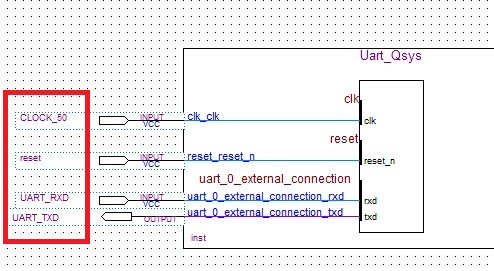
\includegraphics[scale=0.65]{3}
	\caption{Top level entity `Uart\_top.bdf'}
	\label{fig:uart_top}
\end{figure}

\section{NIOS design}
In Chapter \ref{ch:NiosOverview}, we created the `BSP' and `application' file separately for NIOS design. In this chapter, we will use the template provided with NIOS to create the design. For this, open the NIOS software and go to `Files$\rightarrow$New$\rightarrow$NIOS II Application and BSP from Template'. Next, Select the `UART\_Qsys.sopcinfo' file and `Hello World' template and provide the desired name to project e.g. UART\_comm\_app, as shown in Fig , and click `next'. In this window, enter the desired name for BSP file in the `Project name' column e.g. `UART\_comm\_bsp'; and click on Finish.  

\begin{figure}[!h]
	\centering
	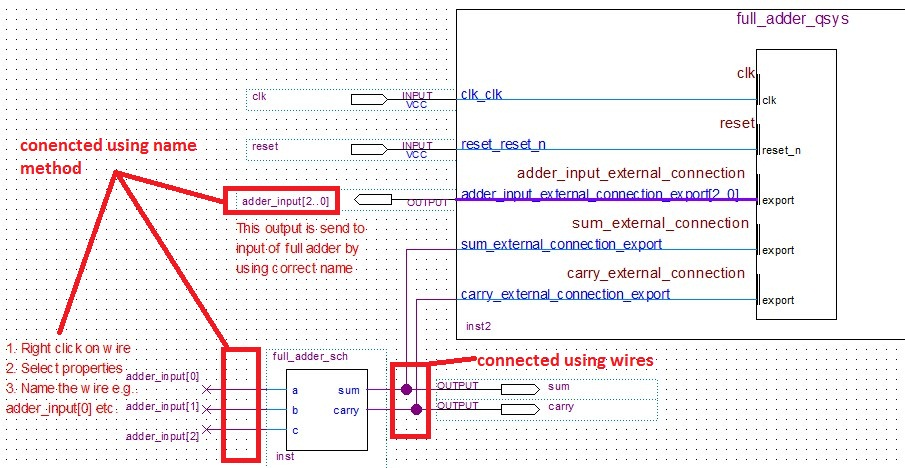
\includegraphics[scale=0.65]{4}
	\caption{Create NIOS project from template}
	\label{fig:nios_name_uart}
\end{figure}

\section{Communication through UART}
To received the data on computer, we need some software like Putty or Tera Term. In this tutorial, we are using `Tera Term software, which can be downloaded freely. Also, we need to change the UART communication settings; so that, we can get messages through UART interface (instead of JTAG-UART)  as shown next. 

Right click on `UART\_comm\_bsp' and go to `NIOS II$\rightarrow$BSP editor'; and select UART\_115200 for various communication as shown in Fig \ref{fig:nios_uart_settings}; and finally click on generate and then click on exit. Now, all the 	`printf' statements will be send to computer via UART port (instead of Jtag-uart). We can change it to JTAG-UART again, by changing UART\_115200 to JTAG-UART again. Note that, when we modify the BSP using BSP-editor, then we need to generate the system again.

\begin{figure}[!h]
	\centering
	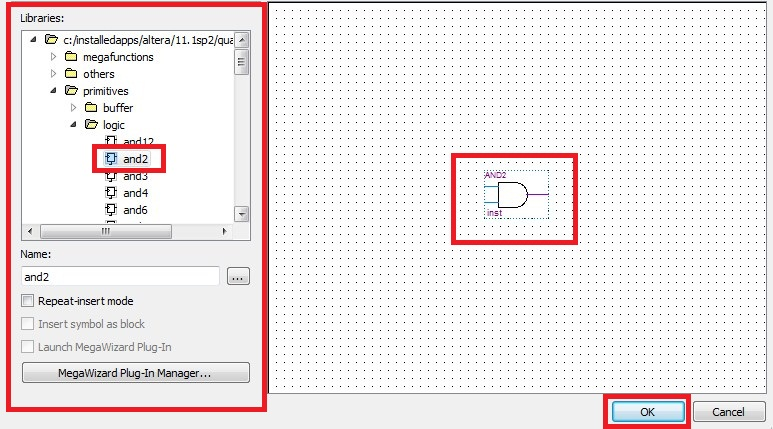
\includegraphics[scale=0.65]{5}
	\caption{UART communication settings in NIOS}
	\label{fig:nios_uart_settings}
\end{figure}

Now, open the Tera Term and select the `Serial' as shown in Fig. \ref{fig:teraTerm}. Then go to `Setup$\rightarrow$Serial Port...' and select the correct baud rate i.e. 115200 and click OK, as shown in Fig. \ref{fig:baudRateteraTerm}. 

\begin{figure}[!h]
	\centering
	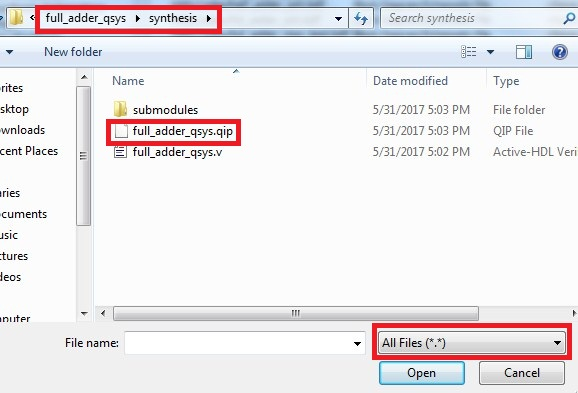
\includegraphics[scale=0.65]{6}
	\caption{Serial communication in Tera Term}
	\label{fig:teraTerm}
\end{figure}

\begin{figure}[!h]
	\centering
	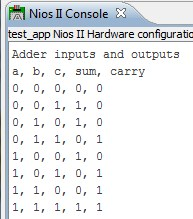
\includegraphics[scale=0.65]{7}
	\caption{Select correct baud rate}
	\label{fig:baudRateteraTerm}
\end{figure}

Finally, right click on `UART\_comm\_app' in NIOS and go to `Run As$\rightarrow$3 NIOS 2 Hardware'. Now, we can see the output on the Tera Term terminal, as shown in Fig. \ref{fig:helloTera}. 

\begin{figure}[!h]
	\centering
	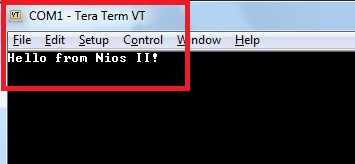
\includegraphics[scale=0.65]{8}
	\caption{`Hello from NIOS II!' on Tera Term}
	\label{fig:helloTera}
\end{figure}

\section{SDRAM Interface}
Our next aim is to generate the Sine waves using NIOS and then plot the waveforms using python. If we write the C-code in current design, then our system will report the memory issue as onchip memory is too small; therefore we need to use external memory. In this section, first, we will update the Qsys design with SDRAM interface, then we will update the Quartus design and finally add the C-code to generate the Sine waves. 

\subsection{Modify QSys}
First, Open the UART\_Qsys.qsys file in QSys software. Now, add SDRAM controller with default settings,  as shown in Fig. \ref{fig:sdram_con}. Next, connect all the ports of SDRMA as shown in Fig. \ref{fig:sdram_connections}. Then, double click the `nios2\_qsys\_0' and select `SDRAM' as reset and exception vector memory, as shown in Fig. \ref{fig:sdram_vector_memory}. 

\begin{figure}[!h]
	\centering
	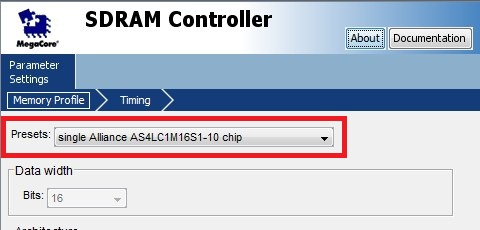
\includegraphics[scale=0.6]{9}
	\caption{SDRAM controller}
	\label{fig:sdram_con}
\end{figure}


\begin{figure}[!h]
	\centering
	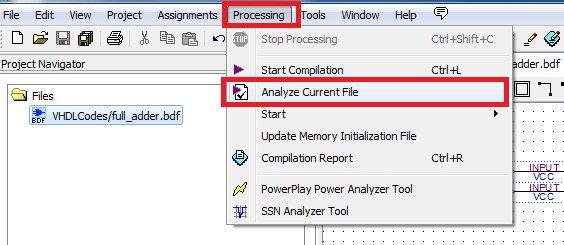
\includegraphics[scale=0.6]{10}
	\caption{SDRAM connections}
	\label{fig:sdram_connections}
\end{figure}


\begin{figure}[!h]
	\centering
	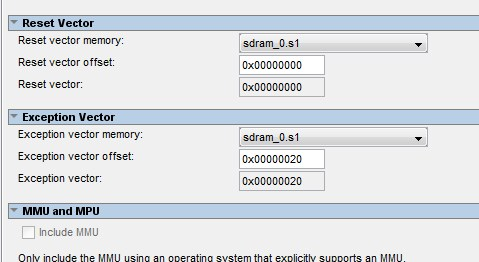
\includegraphics[scale=0.6]{11}
	\caption{Select SDRAM as vector memories}
	\label{fig:sdram_vector_memory}
\end{figure}


Next, we will add `Switches' to control the amplitude of the sine waves. For this add the PIO device of `8 bit with type input', and rename it as `switch', as shown in Fig. \ref{fig:switchForAmplitude} . Finally, go to System$\rightarrow$Assign base addresses, and generate the system. 

\begin{figure}[!h]
	\centering
	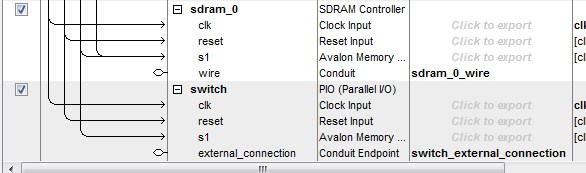
\includegraphics[scale=0.65]{12}
	\caption{Add switches for controlling the amplitude of sine waves}
	\label{fig:switchForAmplitude}
\end{figure}


\subsection{Modify Top level Quartus design}
Now, open the `Uart\_top.bdf' file in Quartus. Right click on the `Uart\_Qsys' block and select `Update symbol or block'; then select the option `Selected symbol(s) or block(s)' and press OK. It will display all the ports for `SDRAM' and switches. Next, we need to assign the correct `pin names' to these ports, as shown in Fig. \ref{fig:SDRAM_Pinassg}.  

\begin{figure}[!h]
	\centering
	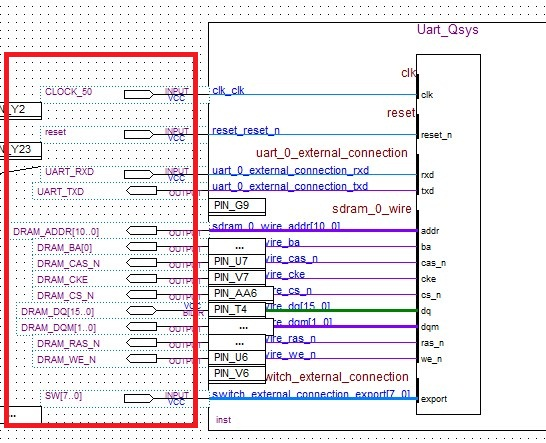
\includegraphics[scale=0.65]{13}
	\caption{Assigning Pins to SDRAM and Switches}
	\label{fig:SDRAM_Pinassg}
\end{figure}

Note that, there should be `-3 ns clock delay' for SDRAM as compare to FPGA clock, therefore we need to add the clock with `-3 ns delay'. For this, double click on the Uart\_top.bdf (anywhere in the file), and select `MegaWizard Plug-In Manager'. Then select `Create a new custom megafunction variation' in the popped-up window and click next. Now, select \textbf{ALTPLL} from \textbf{IO} in \textbf{Installed Plug-Ins} option, as shown in Fig. \ref{fig:dram_clock_altpll}, and click next. Then, follow the figures from Fig. \ref{fig:altpllCreation1} to Fig. \ref{fig:altpllCreation6} to add the ALTPLL to current design i.e. `Uart\_top.bdf'. Finally, connect the ports of this design as shown in Fig. \ref{fig:altpllCreation7}. Note that, in these connections, output of ATLPLL design is connected to `DRAM\_CLK', which is clock-port for DRAM. Lastly, compile and load the design on FPGA board. 

\begin{figure}[!h]
	\centering
	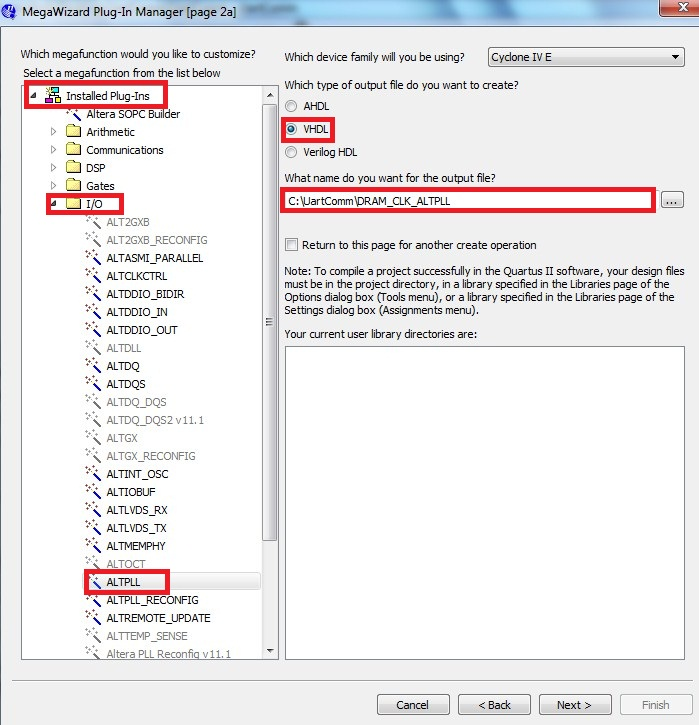
\includegraphics[scale=0.4]{14}
	\caption{ALTPLL generation}
	\label{fig:dram_clock_altpll}
\end{figure}

\begin{figure}[!h]
	\centering
	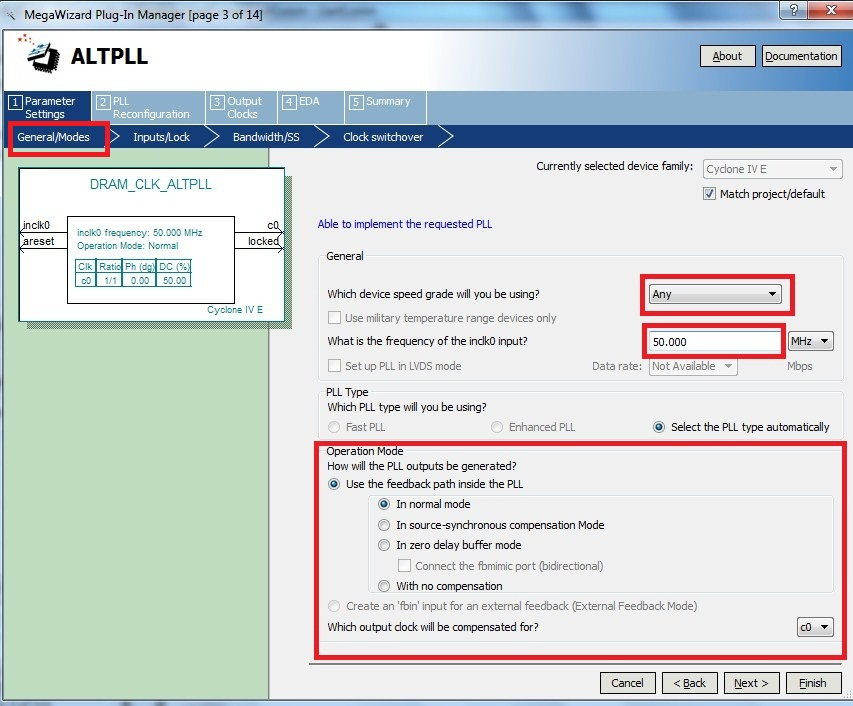
\includegraphics[scale=0.4]{15}
	\caption{ALTPLL creation, step 1}
	\label{fig:altpllCreation1}
\end{figure}

\begin{figure}[!h]
	\centering
	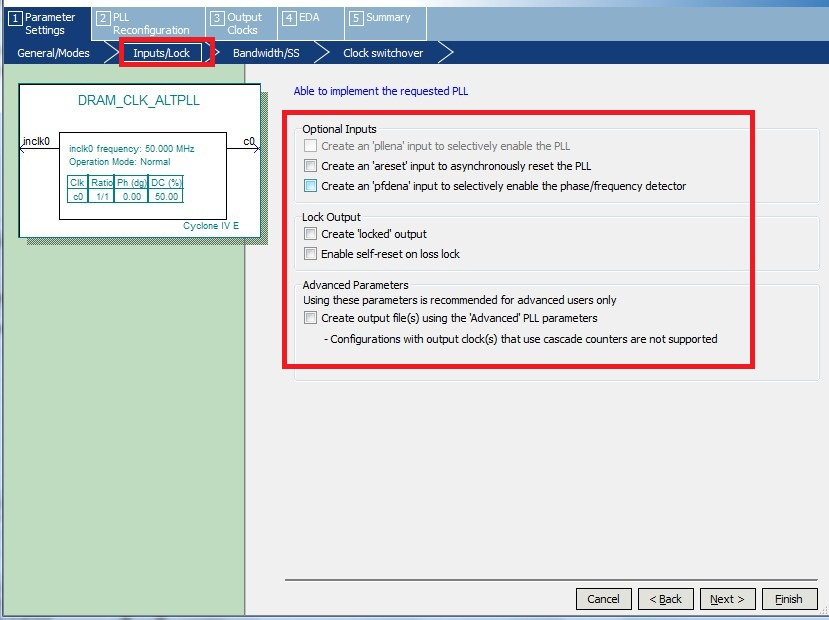
\includegraphics[scale=0.5]{16}
	\caption{ALTPLL creation, step 2}
	\label{fig:altpllCreation2}
\end{figure}

\begin{figure}[!h]
	\centering
	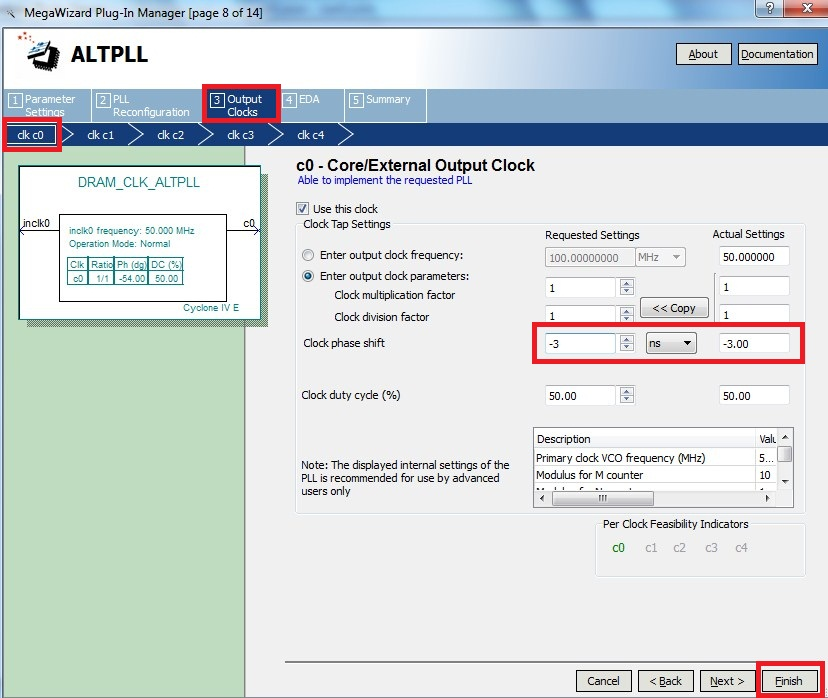
\includegraphics[scale=0.4]{17}
	\caption{ALTPLL creation, step 3}
	\label{fig:altpllCreation3}
\end{figure}

\begin{figure}[!h]
	\centering
	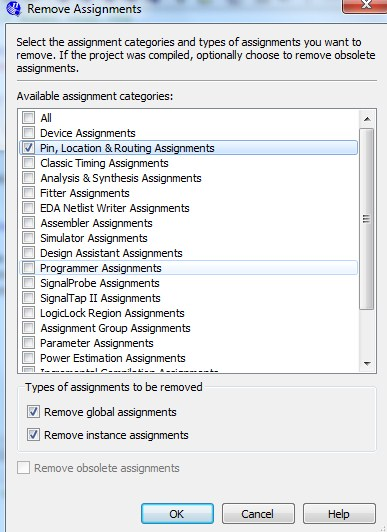
\includegraphics[scale=0.4]{18}
	\caption{ALTPLL creation, step 4}
	\label{fig:altpllCreation4}
\end{figure}

\begin{figure}[!h]
	\centering
	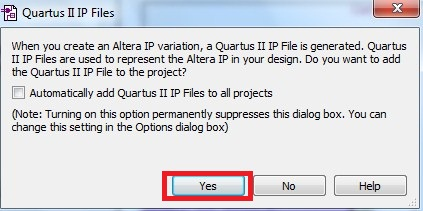
\includegraphics[scale=0.5]{19}
	\caption{ALTPLL creation, step 5}
	\label{fig:altpllCreation5}
\end{figure}

\begin{figure}[!h]
	\centering
	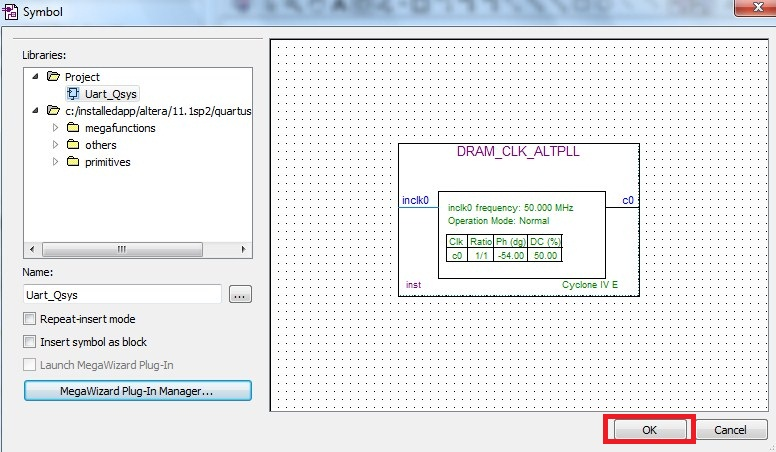
\includegraphics[scale=0.5]{20}
	\caption{ALTPLL creation, step 6}
	\label{fig:altpllCreation6}
\end{figure}

\begin{figure}[!h]
	\centering
	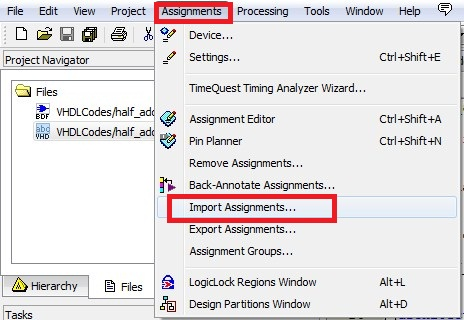
\includegraphics[scale=0.6]{21}
	\caption{Connect ALTPLL design with existing design}
	\label{fig:altpllCreation7}
\end{figure}

\subsection{Updating NIOS design}
Since, we have udpated the QSys design, therefore the corresponding .sopcinfo file is also updated. Further, BSP files depends on the .sopcinfo file, therefore we need to update the BSP as well. For this, right click on `Uart\_comm\_bsp' and go to `NIOS II$\rightarrow$BSP Editor; and update the BSP as shown in Fig. \ref{fig:updateBSPDRAM} and click on `generate' and then click `exit'. Note that, `enable' options are unchecked now, because we are using External memory, which is quite bigger than onchip-memory, so we do not need `small' size options. 

\begin{figure}[!h]
	\centering
	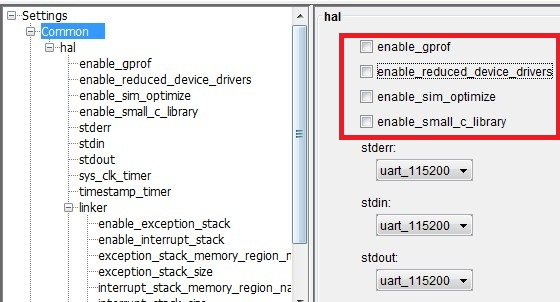
\includegraphics[scale=0.65]{22}
	\caption{Update BSP for new Qsys design}
	\label{fig:updateBSPDRAM}
\end{figure}

Now, update the `hello\_world.c' file as shown in Listing \ref{c:uart_sine_wave}. 

\lstinputlisting[
caption    = {Sin and Cos wave generation},
language = C,
label      = {c:uart_sine_wave}
]{CppCodes/hello_world.c}

In Tera Term, we can save the received values in text file as well. Next, go Files$\rightarrow$Log and select the filename at desired location to save the data e.g. `sineData.txt'. 

Finally, right click on `UART\_comm\_app' in NIOS and go to `Run As$\rightarrow$3 NIOS 2 Hardware'. Now, we can see the decimal values on the screen. If all the switches are at `0' position, then values will be `0.000' as amplitude is zero. Further, we can use any combination of 8 Switches to increase the amplitude of the sine and cosine waves. Also, result will be stored in the  `sineData.txt' file. Content of this file is shown in Fig. \ref{fig:contentLogFile}


\begin{figure}[!h]
	\centering
	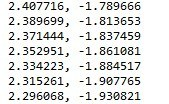
\includegraphics[scale=0.8]{23}
	\caption{Content of `sineData.txt' file}
	\label{fig:contentLogFile}
\end{figure}

\section{Live plotting the data}
In the previous section, we store the sine and cosine wave data on the `sineData.txt' using UART communication. Now, our last task is to plot this data continuously, so that it look line animation. For this save the Listing \ref{pythhon:plotLogData}, in the location where `sineData.txt' is saved. Now, open the command prompt and go to the location of python file. Finally, type \textbf{`python main.py'} and press enter. This will start plotting the waveform continuously based on the data received and stored on the `sineData.txt' file. The corresponding plots are shown in Fig. \ref{fig:plotLogFile}.

\lstinputlisting[
caption    = {Code for live plotting of logged data},
language = Python,
label      = {pythhon:plotLogData}
]{PythonCodes/main.py}

\begin{figure}[!h]
	\centering
	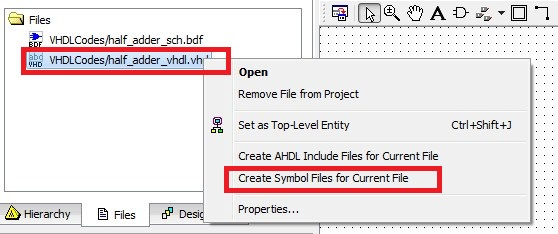
\includegraphics[scale=0.5]{24}
	\caption{Plot of `sineData.txt' file}
	\label{fig:plotLogFile}
\end{figure}


\section{Conclusion}
In this chapter, first we display the `Hello' message using UART and Tera Term. Then, SDRAM is included in the design and correspondingly all the other designs are updated i.e. Quartus and NIOS. Then, the data is stored in the text file and finally it is plotted with the help of Python programming language. 

\section{Introduction}
In Chapter \ref{ch:OverView}, 2-bit comparator is designed using behavior modeling. In that chapter, `if' keyword was used in the `process' statement block. This chapter presents some more such keywords. 

\section{Process block}
All the statements inside the process block execute sequentially. Further, if the architecture contains more than one process block, then all the process blocks execute in parallel, i.e. process blocks are the concurrent blocks. 

\begin{noNumBox}
	Note that, we can write the complete design using sequential programming. But that may result in very complex hardware design, or to the design which can not be synthesized at all. The best way of designing is to make small units using behavioral and dataflow modeling, and then use the structural modeling style to create the large system. 
\end{noNumBox}

\section{If-else statement}
In this section, 4$\times$1 multiplexed is designed using If-else statement. We already see the working of `if' statement in Chapter \ref{ch:OverView}. In lines of 17-27 of Listing \ref{vhdl:ifEx}, `elsif' and `else' are added to `if' statement. Note that, If-else block can contain multiple `elsif' statements between one `if' and one `else' statement. Further, `null' is added in line 26 of Listing \ref{vhdl:ifEx}, whose function is same as `unaffected' in concurrent signal assignment as shown in Listing \ref{vhdl:multiplexerVhdl}. Fig. \ref{fig:ifExWave} shows the waveform generated by Modelsim for Listing \ref{vhdl:ifEx}. 

\begin{noNumBox}
	Note : 
	\begin{enumerate}
		\item The `multiplexer design' in Fig. \ref{fig:ifEx} (generated by if-else in Listing \ref{vhdl:ifEx}) is exactly same as the design in Fig. \ref{fig:multiplexerEx} (generated by when-else in Listing \ref{vhdl:multiplexerEx}).  
		
		\item Further, in Section \ref{sec:concurrentSeq}, it is said that the `combinational logic can be implemented using both the concurrent statements and the sequential statements. Note that, the multiplexer is the `combinational design' as the output depends only on current input values. And it implemented using `concurrent statements' and `sequential statements' in Listing \ref{vhdl:multiplexerEx} and Listing \ref{vhdl:ifEx} respectively. 
	\end{enumerate}
\end{noNumBox}
\lstinputlisting[
language = Vhdl,
caption    = {Multiplexer using if statement},
label      = {vhdl:ifEx}
]{ifEx.vhd}
\begin{figure}
	\centering
	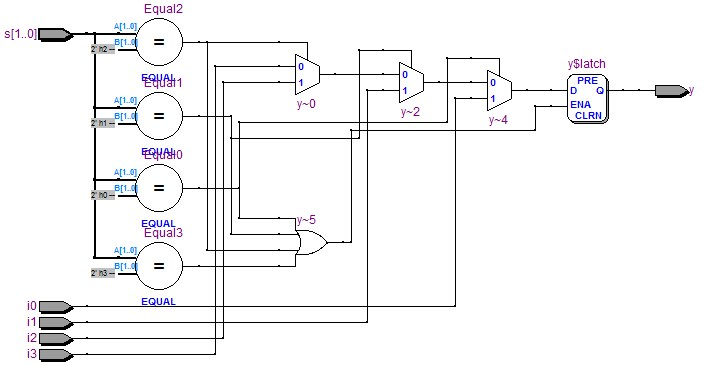
\includegraphics[width=0.8\textwidth]{ifEx}
	\caption{Multiplexer using if statement, Listing \ref{vhdl:ifEx}}
	\label{fig:ifEx}
\end{figure}
\begin{figure}
	\centering
	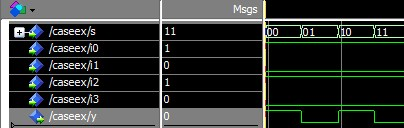
\includegraphics[scale=1]{ifExWave}
	\caption{Waveforms of Listing \ref{vhdl:ifEx} and \ref{vhdl:caseEx}}
	\label{fig:ifExWave}
\end{figure}


\section{Case statement}
Case statement is shown in lines 17-28 of Listing \ref{vhdl:caseEx}. `s' is defined in case statement at line 17; whose value is checked using `when' keyword at lines 18 and 20 etc. The value of `y' depends on the value of `s' e.g. if `s' is ``01'', then line 20 will be true, hence value of `i1' will be assigned to `y'. 

\begin{noNumBox}
	Note that the `multiplexer design' in Fig. \ref{fig:caseEx} (generated by case in Listing \ref{vhdl:caseEx}) is exactly same as the design in Fig. \ref{fig:multiplexerVhdl} (generated by with-select in Listing \ref{vhdl:multiplexerVhdl}). 
\end{noNumBox}


\lstinputlisting[
language = Vhdl,
caption    = {Multiplexer using case statement},
label      = {vhdl:caseEx}
]{caseEx.vhd}
\begin{figure}
	\centering
	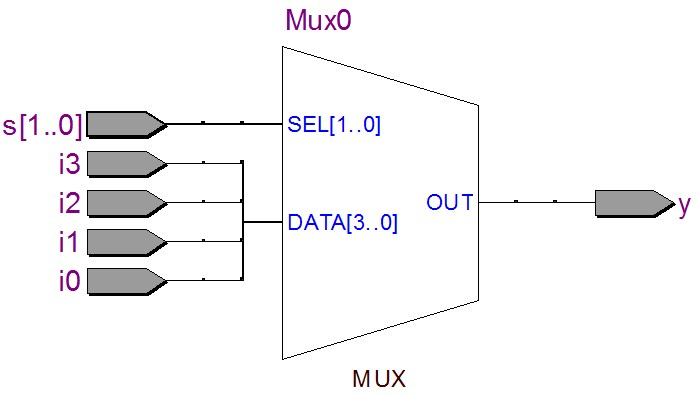
\includegraphics[scale=0.4]{caseEx}
	\caption{Multiplexer using case statement, Listing \ref{vhdl:caseEx}}
	\label{fig:caseEx}
\end{figure}

\section{Wait statement}
`Wait statement' is used to hold the system for certain time duration. It can be used in three different ways as shown below, 

\begin{enumerate}
	\item \textbf{wait until} : It is \textbf{synthesizable} statement and holds the system until the defined condition is met e.g. ``wait until clk = '1''' will hold the system until clk is `1'. 
	
	\item \textbf{wait on} : It is \textbf{synthesizable} statement and holds the system until the defined signal is changed e.g. `wait on clk' will hold the system until clk changes it's value i.e. `0' to `1' or vice-versa.
	
	\item \textbf{wait for} : It is \textbf{not synthesizable} and holds the system for the defined timed e.g. `wait for 20ns' will hold the system for 20 ns. This is used with testbenches as shown in Chapter \ref{ch:Testbench}.
\end{enumerate}

\section{Problem with Loops}

VHDL provides two loop statements i.e. `for' loop and `while' loop'. These loops are very different from software loops. Suppose `for i = 1 to N' is a loop, then, in software `i' will be assigned one value at a time i.e. first i=1, then next cycle i=2 and so on. Whereas in VHDL, N logic will be implement for this loop, which will execute in parallel. Also, in software, `N' cycles are required to complete the loop, whereas in VHDL the loop will execute in one cycle. 
\begin{noNumBox}
	As loops implement the design-units multiple times, therefore design may become large and sometimes can not be synthesized as well. If we do not want to execute everything in one cycle (which is almost always the case), then loops can be replaced by `case' statements and `conditional' statements as shown in section \ref{sec:ifLoop}. Further, due to these reasons, we do not use loops for the design. Lastly, the loops can be extremely useful in testbences, when we want to iterate through all the test-data which is shown in Listing \ref{vhdl:half_adder_lookup_tb.vhd}.  
\end{noNumBox}   

\section{Loop using `if' statement}\label{sec:ifLoop}
In Listing \ref{vhdl:ifLoop}, a loop is created using `if' statement, which counts the number upto input `x'. 

\begin{explanation}[Listing \ref{vhdl:ifLoop}]
	In the listing, two `process' blocks are used i.e. at lines 20 and 31. The process at line 20 checks whether the signal `count' value is `less or equal' to input x (line 22), and sets the currentState to `continueState'; otherwise if count is greater than the input x, then currentState is set to `stopState'.
	
	Then next process statement (line 31), increase the `count' by 1, if currentState is `continueState'; otherwise count is set to 0 for stopState. Finally count is displayed at the output through line 39. In this way, we can implement the loops using process statements. 
	
	Fig. \ref{fig:ifLoop} shows the loop generated by the listing with generic value N=1. Further,  Fig. \ref{fig:ifLoopWave} shows the count-waveforms generated by the listing with generic value N = 3.
	
	\textbf{Sensitivity list of the process block should be implemented carefully. For example, if we add `count' in the sensitivity list at line 31 of Listing  \ref{vhdl:ifLoop}, then the process block will execute infinite times. This will occur because the process block execute whenever there is any event in the signals in the sensitivity list; therefore any change in `count' will execute the block, and then this block will change the `count' value through line 34. Since `count' value is changed, therefore process block will execute again, and the loop will never exit.}
	
\end{explanation}

\lstinputlisting[
language = Vhdl,
caption    = {Loop using `if' statement},
label      = {vhdl:ifLoop}
]{ifLoop.vhd}
\begin{figure}[!h]
	\centering
	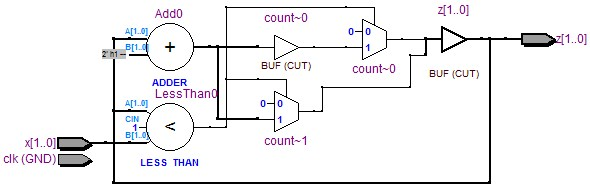
\includegraphics[width=\textwidth]{ifLoop}
	\caption{Loop using `if' statement, Listing \ref{vhdl:ifLoop} with N = 1}
	\label{fig:ifLoop}
\end{figure}

\begin{figure}[!h]
	\centering
	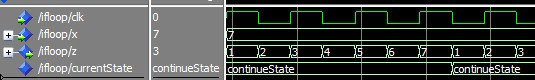
\includegraphics[width=\textwidth]{ifLoopWave}
	\caption{Loop using `if' statement, Listing \ref{vhdl:ifLoop} with N = 3}
	\label{fig:ifLoopWave}
\end{figure}

\begin{noNumBox}
	Note that, the design in Listing \ref{vhdl:ifLoop} is not good because of following reasons,
	\begin{enumerate}		
		\item First, the clock is used in the sensitive list, therefore it may arise race-around condition in the system. To avoid it, the system should be sensitive to only edge of the clock (i.e. positive and negative) , which is discussed in Listing \ref{vhdl:BasicDFF} using `event' keyword.
		
		\item Secondly, the process statement in Line 31, does not required the `clk' in the sensitive list. In Fig. \ref{fig:combSeqBlock}, we saw that the sequential designs contain both `combinational logic' and `sequential logic'; also the figure shows that the `clock' is required  only for `sequential logics'. But in the current design, we used clock in both `combinational logic' and `sequential logic'. Detailed discussion about FSM designs are in Chapter \ref{ch:FSM}, where such issues are raised for careful designs.  
	\end{enumerate}
	
\end{noNumBox}

\section{Conclusion}
In this chapter, various statements of behavioral modeling styles are discussed. Also, we saw the relationship between the designs generated by behavior modeling and dataflow modeling. Further, problem with loops are discussed and finally loop is implemented using `if' statement. 